\documentclass[a4paper]{article}
\usepackage[utf8x]{inputenc}
\usepackage[T1,T2A]{fontenc}
\usepackage[russian]{babel}
\usepackage{hyperref}
\usepackage{indentfirst}
\usepackage{color}
\usepackage{listings}
\usepackage{here}
\usepackage{array}
\usepackage{multirow}
\usepackage{graphicx}
\usepackage{caption}

\lstset{ %
extendedchars=\true,
keepspaces=true,
language=C++,					% choose the language of the code
basicstyle=\footnotesize,		% the size of the fonts that are used for the code
numbers=left,					% where to put the line-numbers
numberstyle=\footnotesize,		% the size of the fonts that are used for the line-numbers
stepnumber=1,					% the step between two line-numbers. If it is 1 each line will be numbered
numbersep=5pt,					% how far the line-numbers are from the code
backgroundcolor=\color{white},	% choose the background color. You must add \usepackage{color}
showspaces=false				% show spaces adding particular underscores
showstringspaces=false,			% underline spaces within strings
showtabs=false,					% show tabs within strings adding particular underscores
frame=single,           		% adds a frame around the code
tabsize=4,						% sets default tabsize to 2 spaces
captionpos=b,					% sets the caption-position to bottom
breaklines=true,				% sets automatic line breaking
breakatwhitespace=false,		% sets if automatic breaks should only happen at whitespace
escapeinside={\%*}{*)},			% if you want to add a comment within your code
postbreak=\raisebox{0ex}[0ex][0ex]{\ensuremath{\color{red}\hookrightarrow\space}}
}
\begin{document}	% начало документа


\begin{titlepage}	% начало титульной страницы

	\begin{center}		% выравнивание по центру

		\large Санкт-Петербургский Политехнический Университет Петра Великого\\
		\large Институт компьютерных наук и технологий \\
		\large Кафедра компьютерных систем и программных технологий\\[6cm]
		% название института, затем отступ 6см
		
		\huge Программирование\\[0.5cm] % название работы, затем отступ 0,5см
		\large Отчет по курсовой работе\\[0.1cm]
		\large "Жизнь"\\[5cm]

	\end{center}


	\begin{flushright} % выравнивание по правому краю
		\begin{minipage}{0.25\textwidth} % врезка в половину ширины текста
			\begin{flushleft} % выровнять её содержимое по левому краю

				\large\textbf{Работу выполнил:}\\
				\large Корсков А.В.\\
				\large {Группа:} 13501/4\\
				
				\large \textbf{Преподаватель:}\\
				\large Вылегжанина К.Д.
				

			\end{flushleft}
		\end{minipage}
	\end{flushright}
	
	\vfill % заполнить всё доступное ниже пространство

	\begin{center}
	\large Санкт-Петербург\\
	\large \the\year % вывести дату
	\end{center} % закончить выравнивание по центру

\thispagestyle{empty} % не нумеровать страницу
\end{titlepage} % конец титульной страницы

\vfill % заполнить всё доступное ниже пространство
% Содержание
\tableofcontents
\newpage

\section{Модель Жизнь}
\subsection{Задание}
Жизнь. Из файла считывается прямоугольное поле, каждая клетка которого либо жива, либо мертва. В очередном поколении, мертвая клетка становится живой, если она имела ровно трех живых соседей, в противном случае остается мертвой. Живая клетка остается живой, если она имела двух или трех живых соседей, в противном случае становится мертвой. Реализовать на экране процесс смены поколений. Программа должна позволять сохранять вид игрового поля для использования его в будущем.

\subsection{Правила работы программы}
В редакторе последовательно сменяются поколения. Программа проверяет у каждой клетки состояния всех соседних клеток. Если у мёртвой клетки три живых соседа, то клетка поменяет свой статус на живой, иначе останется мёртвой. То же самое происходит и у живой клетки, она остаётся живой если два или три соседа живые, иначе становится мёртвой. Ещё одним принципиальным правилом является наличие функции сохранения в файл и загрузки из файла поля с зафиксированным состояние всех клеток.

\subsection{Концепция}
Готовый проект должен моделировать превращение живых клеток в мёртвые и наоборот. Эти превращения проходят по определённым правилам. Пользователь должен иметь возможность наблюдать за текущим состоянием поля и превращением клеток. Также важной функцией программы является возможность сохранить текущее состояние поля в файл и загрузка поля из файла. 

\subsection{Минимально работоспособный продукт}
Минимально работоспособный продукт должен уметь: предоставить пользователю информацию о текущем состоянии клеток, сохранение и загрузка поля в файл.


\subsection{Диаграмма прецедентов использования}

\begin{figure}[H]
	\begin{center}
		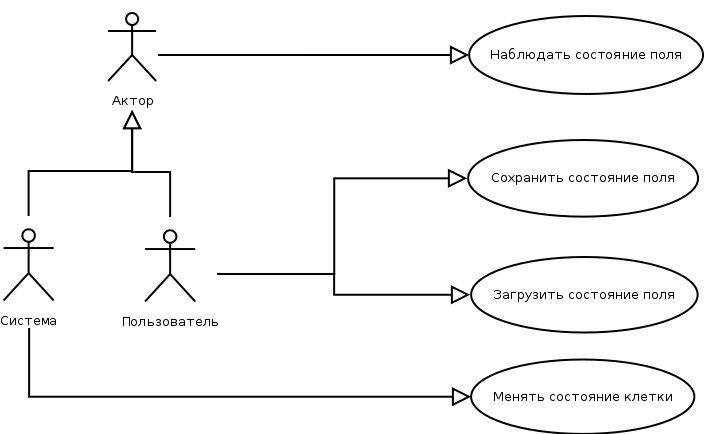
\includegraphics[scale=0.4, height=7cm]{Diagrams/Diagram1}
		\caption{Диаграмма прецедентов использования} 
		\label{pic:Diagram1} % название для ссылок внутри кода
	\end{center}
\end{figure}

\section{Проектрование приложения, реализующего модель Жизнь}
Программа разделена на 4 подпроекта: app - консольное приложение, core - библиотека, реализующая модель Жизнь, gui - графическое приложение, test - тесты для программы.

\begin{figure}[H]
	\begin{center}
		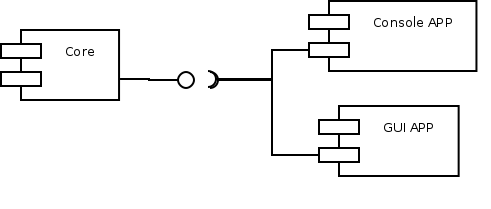
\includegraphics[scale=0.4, height=7cm]{Diagrams/Diagram2}
		\caption{Диаграмма прецедентов использования} 
		\label{pic:Diagram2} % название для ссылок внутри кода
	\end{center}
\end{figure}

\subsection{Библиотека}
При написании проекта, была создана библиотека. В ней находятся все необходимые классы для создания и работы модели. Один из классов (api) создан для предоставления всех действий над моделью.

\noindent В API выделены следующие методы: 
\begin{itemize}
\item initialize\_settings - метод, задающий размеры поля.
\item initialize\_field - метод, инициализирующий поле случайными клетками.
\item save\_field - метод, сохраняющий поле в файл.
\item load\_field - метод, загружающий поле из файла.
\item print\_field - метод, выводящий поле в консоль.
\item change\_field - метод, меняющий поколение на следующее.
\item set\_cell - метод, задающий клетку на поле. 
\end{itemize}


\section{Реализация модели Жизнь}
\subsection{Версии программ}
Операционная система: Debian 8.1, среда разработки: Qt Creator 3.5.0, компилятор: GCC 4.9.1, система документирования: Doxygen 1.8.8, Qt 5.5.0.

\subsection{Консольное приложение}
Консольное приложение позволяет работать с моделью через консоль.

\noindent Основные классы, выделенные в консольном приложении:
\begin{itemize}
\item Класс console\_ui. Сначала выводит главное меню, где можно создать модель или загрузить. Также есть метод выводящий второе меню, где можно запустить следующее поколение или сохранить модель и в третьем меню можно задать размер поля. 
\end{itemize}

\begin{figure}[H]
	\begin{center}
		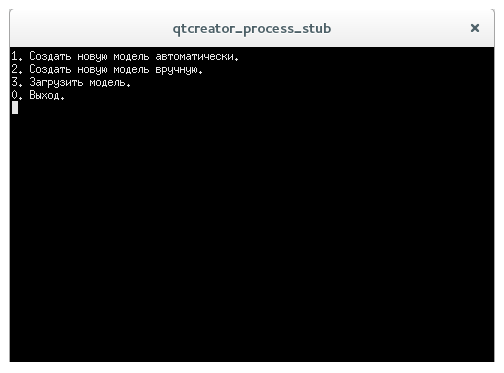
\includegraphics[scale=0.5]{console}
		\caption{Главное меню консольного приложения} 
		\label{pic:console} % название для ссылок внутри кода
	\end{center}
\end{figure}

На рис \ref{pic:console} представлено главное меню приложения. Есть возможность создать новую модель случайными клетками, создать модель вручную, загрузить модель из файла и выйти из программы. 

\begin{figure}[H]
	\begin{center}
		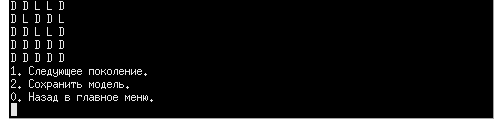
\includegraphics[scale=0.5]{console2}
		\caption{Поле и второе меню в консольном приложении} 
		\label{pic:secondMenu} % название для ссылок внутри кода
	\end{center}
\end{figure}

На рис \ref{pic:secondMenu} показано поле и внизу меню, в котором можно сменить поколение, сохранить поле или вернуться в главное меню.

\begin{figure}[H]
	\begin{center}
		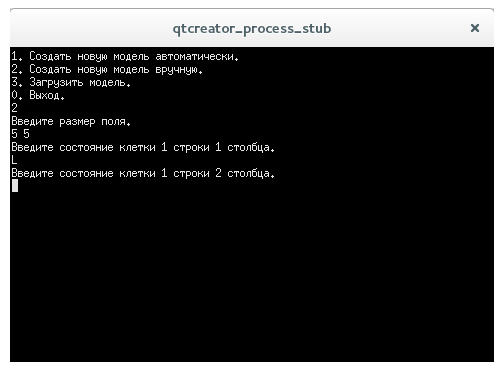
\includegraphics[scale=0.5]{console3}
		\caption{Поле модели в консольном приложении} 
		\label{pic:cellMenu} % название для ссылок внутри кода
	\end{center}
\end{figure}

На рис \ref{pic:cellMenu} показано главное меню ниже расположено меню размера поля и в самом низу два меню ввода состояния клеток. 

\subsection{Библиотека}
\noindent Основные классы, выделенные в библиотеке:
\begin{itemize}
\item Класс Cell. Реализует клетку. Содержит координаты клетки и её состояние. Присутствуют методы, возвращающие и задающие координаты и состояние клетки. Также есть метод, проверяющий сколько живых соседей у данной клетки.
\item Класс Field. Класс представляет поле модели. Содержит размер поля и двумерный массив клеток. Присутствуют методы, возвращающие и задающие размер поля, отдельную клетку и весь двумерный массив клеток.	
\item Класс Api. Класс, предоставляющий все методы, доступные над моделью. Позволяет задать размер поля, инициализировать поле случайными клетками, задать отдельную клетку, сохранить и загрузить поле из файла и вывести его.
\end{itemize}

\subsection{Графическое приложение}
Графическое приложение позволяет работать с моделью через окна графического приложения.

\noindent Основные классы, выделенные в графическом приложении. 
\begin{itemize}
\item Класс MainWindow. Главное окно приложения. Присутствуют кнопки «Создать новую случайную модель», «Создать новую модель вручную», «Загрузить модель», «Сделать модель с фигурой», «Выход».
\item Класс exit\_window. Окно для полтверждения выхода.
\item Класс field\_window. Окно отображающее поле. Присутствуют кнопки «Следующее поколение», «Сохранить модель», «Назад в главное меню».
\item Класс figure\_window. Окно позволяющее выбрать готовое поле. Присутствуют кнопки «Глайдер» и «Космический корабль».
\item Класс initialize\_window. Окно позволяющее выбрать состояние поле. Присутствуют кнопки «Живая» и «Мёртвая».
\item Класс size\_window. Окно позволяющее задать размер поля.
\end{itemize}

\begin{figure}[H]
	\begin{center}
		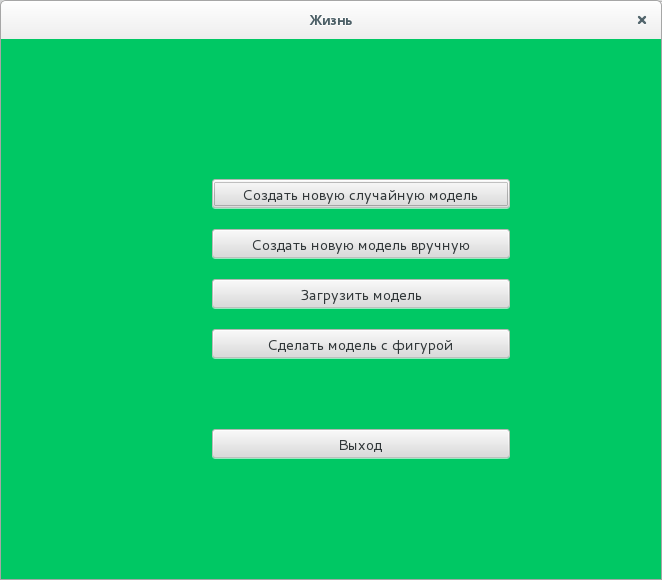
\includegraphics[scale=0.5]{gui}
		\caption{Главное меню графического приложения} 
		\label{pic:graphicsMeinMenu} % название для ссылок внутри кода
	\end{center}
\end{figure}

На рис \ref{pic:graphicsMeinMenu} представлено главное окно приложения. В нём пользователю можно создать поле случайными клетками, вручную, загрузить из файла, создать поле с готовыми фигурами или выйти из программы. 

\begin{figure}[H]
	\begin{center}
		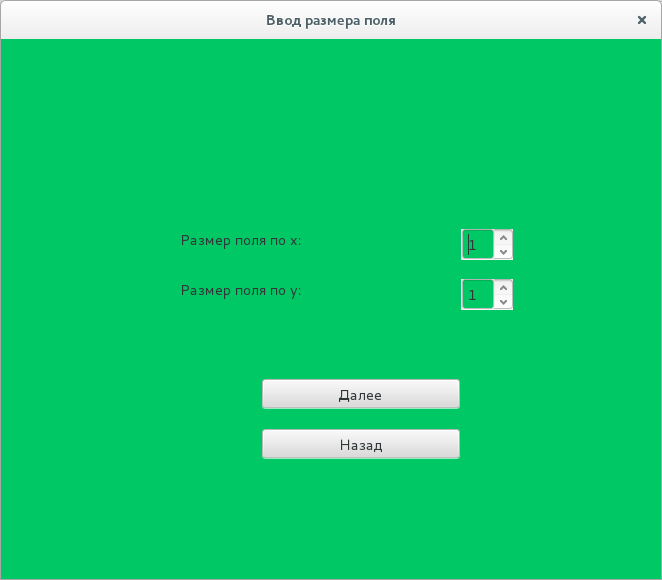
\includegraphics[scale=0.5]{gui2}
		\caption{Настройки модели в графическом приложении} 
		\label{pic:graphicsSizeMenu} % название для ссылок внутри кода
	\end{center}
\end{figure}

На рис \ref{pic:graphicsSizeMenu} – окно выбора размера приложения.

\begin{figure}[H]
	\begin{center}
		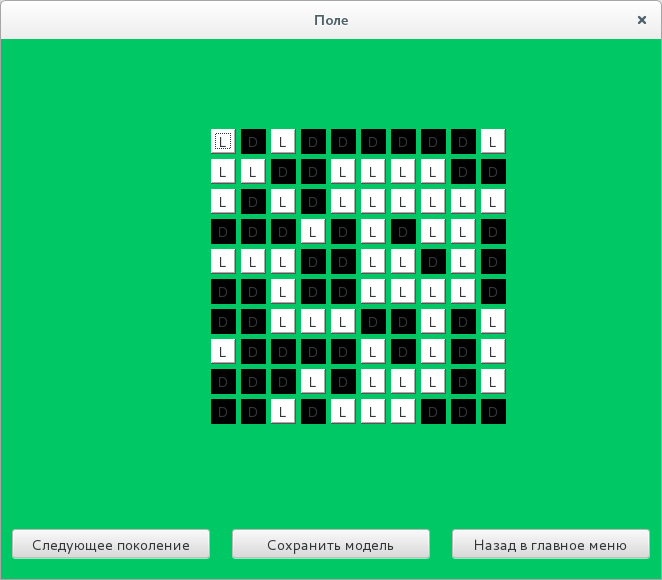
\includegraphics[scale=0.5]{gui3}
		\caption{Представление поля в графическом приложении} 
		\label{pic:field} % название для ссылок внутри кода
	\end{center}
\end{figure}

На рис \ref{pic:field} – окно с полем, внизу есть кнопки для запуска следующего поколения, сохранения модели и выхода в главное меню.

\section{Процесс обеспечения качества и тестирование}
\subsection{Тестирование}
Приложение содержит автоматические тесты. Протестированы некоторые основные функции. Проверяется назначение поля размера, заполнение его случайными клетками и правильность получения следующего поколения.

\section{Вывод}
По окончании семестра автор проекта научился делать графический интерфейс с помощью Qt, а также получил опыт работы с большими проектами, содержащими много классов и имеющих как консольное приложение, так и графическое.

\section{Приложение 1. Листинги кода}
\subsection{Консольное приложение}
\lstinputlisting[]
{../sources/livingcells/app/main.cpp}
\newpage

\lstinputlisting[]
{../sources/livingcells/app/console_ui.h}
\lstinputlisting[]
{../sources/livingcells/app/console_ui.cpp}
\newpage

\subsection{Графическое приложение}
\lstinputlisting[]
{../sources/livingcells/gui/main.cpp}
\newpage

\lstinputlisting[]
{../sources/livingcells/gui/exit_window.h}
\lstinputlisting[]
{../sources/livingcells/gui/exit_window.cpp}
\newpage

\lstinputlisting[]
{../sources/livingcells/gui/field_window.h}
\lstinputlisting[]
{../sources/livingcells/gui/field_window.cpp}
\newpage

\lstinputlisting[]
{../sources/livingcells/gui/figure_window.h}
\lstinputlisting[]
{../sources/livingcells/gui/figure_window.cpp}
\newpage

\lstinputlisting[]
{../sources/livingcells/gui/initialize_window.h}
\lstinputlisting[]
{../sources/livingcells/gui/initialize_window.cpp}
\newpage

\lstinputlisting[]
{../sources/livingcells/gui/mainwindow.h}
\lstinputlisting[]
{../sources/livingcells/gui/mainwindow.cpp}
\newpage

\lstinputlisting[]
{../sources/livingcells/gui/size_window.h}
\lstinputlisting[]
{../sources/livingcells/gui/size_window.cpp}
\newpage

\subsection{Библиотека}

\lstinputlisting[]
{../sources/livingcells/core/api.h}
\lstinputlisting[]
{../sources/livingcells/core/api.cpp}
\newpage

\lstinputlisting[]
{../sources/livingcells/core/cell.h}
\lstinputlisting[]
{../sources/livingcells/core/cell.cpp}
\newpage

\lstinputlisting[]
{../sources/livingcells/core/field.h}
\lstinputlisting[]
{../sources/livingcells/core/field.cpp}
\newpage

\subsection{Тесты}

\lstinputlisting[]
{../sources/livingcells/test/tst_testtest.cpp}
\newpage
\end{document}